\documentclass[border=0pt, tikz]{standalone}
\usepackage{tikz}

\begin{document}
    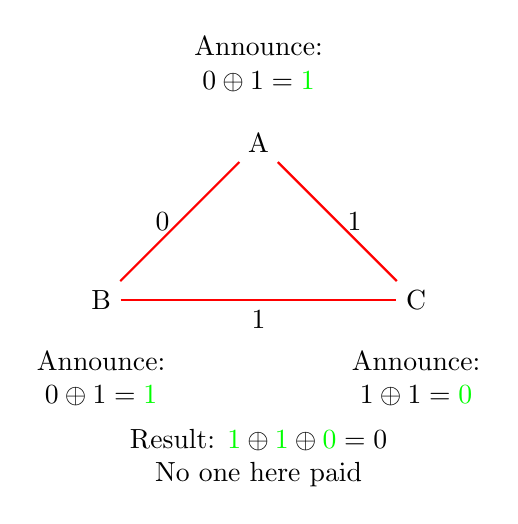
\begin{tikzpicture}[node distance = 2cm]
        \node (A) {A};
        \node [left of = A, below of = A] (B) {B};
        \node [right of = A, below of = A] (C) {C};

        \draw [thick, red] (A)--(B) node [midway, above, left] {
        \textcolor{black}0};
        \draw [thick, red] (B)--(C) node [midway, below] {\textcolor{black}1};
        \draw [thick, red] (C)--(A) node [midway, above, right] {
        \textcolor{black}1};

        \node [align=center,above of = A, node distance = 1cm] (_) 
        {Announce:\\$0\oplus 1 = \textcolor{green}1$};
        \node [align=center, below of = B, node distance = 1cm] (_) 
        {Announce:\\$0\oplus 1 = \textcolor{green}1$};
        \node [align=center, below of = C, node distance = 1cm] (_) 
        {Announce:\\$1\oplus 1 = \textcolor{green}0$};

        \node [align=center, below of = C, left of = C] (_) {Result: 
        $\textcolor{green}1\oplus \textcolor{green}1\oplus \textcolor{green}0 =
        0$\\\textcolor{black}No one here paid};
    \end{tikzpicture}
\end{document}
